\documentclass[11pt]{article}

\usepackage{float}
\usepackage{hyperref}
\usepackage{fullpage}
\usepackage{verbatim}
\usepackage{moreverb}
\usepackage{graphicx}
\usepackage{array}
\usepackage{booktabs}
\usepackage{parskip}
\usepackage{tikz}
\usetikzlibrary{arrows,automata, positioning}
\usepackage{minted}
\let\verbatiminput=\verbatimtabinput
\def\verbatimtabsize{4\relax}
\graphicspath{{images/}}

\begin{document}
\title{EECS 151/251A FPGA Lab\\
Lab 6: AC97 (Audio) Controller and FPGA - IC Communication}

\author{Prof. Borivoje Nikolic \\
TA: Vighnesh Iyer \\Department of Electrical Engineering and Computer Sciences\\
College of Engineering, University of California, Berkeley}
\date{}
\maketitle

\tableofcontents

\section{Before You Start This Lab}

These documents will be helpful as you work through this lab.

\begin{enumerate}
	\item \textbf{labs\_fa16/docs/AC97\_Spec.pdf}
	
	The official specification of the AC97 protocol which you will partially implement in this lab. This is a large document but there are only a few sections that are important to us. They will be referenced later in the spec.
	
	\item \textbf{labs\_fa16/docs/AD1981B\_Datasheet.pdf}
	
	The datasheet of the AD1981B AC97 Audio Codec. We will be writing a controller that lives on the FPGA which will communicate with this IC using the AC97 protocol. This IC receives audio data over the AC97 protocol and converts the digital audio data to an analog signal which is sent through the headphone jack.
\end{enumerate}

\textbf{We strongly recommend you read through this entire document before coming to lab.}

\section{Lab Overview}
Run \verb|git pull| in your \textbf{git cloned} \verb|labs_fa16| directory to \textbf{fetch the latest skeleton files for this lab.}

In this lab, we will create a AC97 controller that lives on the FPGA. The controller will interact with an AC97 audio codec IC on the ML505 development board. Your controller will implement a portion of the AC97 protocol that will allow it to send digital audio data and control signals to the IC.

\textbf{This lab will be done in teams of two; it will involve building a peripheral used later in the project.}

\section{Introduction to the AC97 Protocol}
AC97 is a protocol which is used for communication between a source/producer of audio data and an audio codec. The audio codec present on the FPGA development board (ML505) is the Analog Devices AD1981B Codec. Our processor will send digital packets to this codec using the AC97 protocol.

Refer to the AD1981B Codec datasheet and the official AC97 spec when working through this lab. They are in the \verb|labs_fa16/docs| folder.

\subsection{Protocol Connections}

\begin{figure}[H]
	\begin{center}
		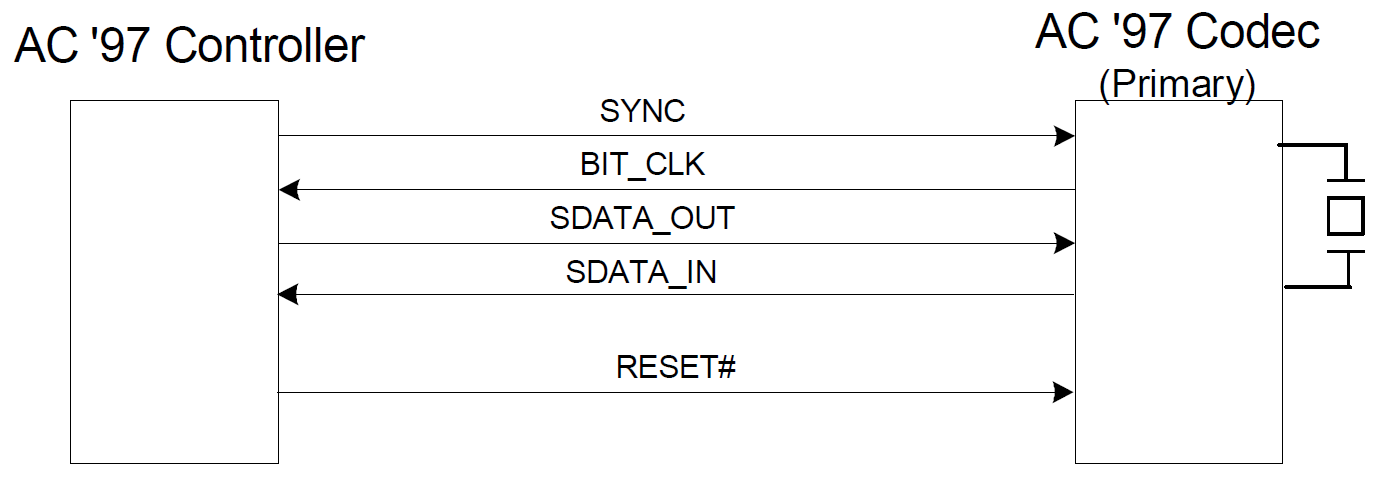
\includegraphics[width=6in]{ac97_connections}
		\caption{Codec - Controller Connections}
	\end{center}
\end{figure}

There are 5 wires involved in the AC97 protocol. They are

\begin{enumerate}
	\item \verb|SYNC| - tells the codec when a frame is about to start
	\item \verb|BIT_CLK| - a clock from the codec which your controller should synchronize its data transfers with
	\item \verb|SDATA_OUT| - the serial line on which your controller transmits data to the codec
	\item \verb|SDATA_IN| - the serial line on which the codec transmits data to your controller (not used in this lab)
	\item \verb|RESET#| - a signal used by your controller to reset the codec
\end{enumerate}

The way in which your controller transmits audio samples (linear PCM) to the codec is through the \verb|SDATA_OUT| wire. There is a specific method of framing the samples so that the codec knows how to read them which is defined by the AC97 spec.

\subsection{How Data is Transmitted}
AC97 is a \textbf{serial interface}: data is transmitted to and from the codec one bit at a time. On every cycle of the AC97 bit clock (\verb|BIT_CLK|), one bit of data is transfered from the AC97 controller (on the FPGA) to the codec over the \verb|SDATA_OUT| wire, and one bit of data is transfered from the codec to the FPGA over the \verb|SDATA_IN| wire.

The constant streams of data passing between the codec and the FPGA are divided into frames. The bit clock is generated by the codec, and runs at 12.288MHz. There are 256 bits per frame, so 48,000 frames are sent per second. This is where the 48kHz sampling rate of the codec comes from. Each frame sent to the codec provides one 20-bit audio sample for each of the DACs in the codec, and each frame sent by the codec provides one 20-bit sample from each of the codec's ADCs.

Frames are divided into twelve slots of 20 bits each, plus a 16-bit tag field, which serves as the frame header. Each slot serves a different purpose and contains various types of data to be sent to the codec. Each slot should be sent with the MSB first going down to the LSB. For example if you were to send \verb|data[19:0]| in slot 1, you would begin by sending \verb|data[19]| and finish by sending \verb|data[0]|.

The start of each frame is indicated by a rising edge of the SYNC signal. The SYNC signal goes high one clock cycle before the first bit of a frame, and goes low at the same time as the last bit of the tag field is sent. The diagrams below will summarize how frames are sent using the AC97 protocol.

\begin{figure}[hbt]
	\begin{center}
		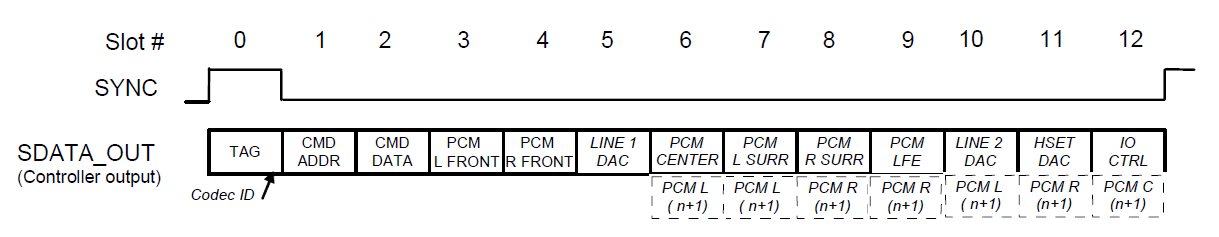
\includegraphics[width=6in]{ac97_framing}
		\caption{Framing for AC97}
	\end{center}
\end{figure}

\begin{figure}[hbt]
	\begin{center}
		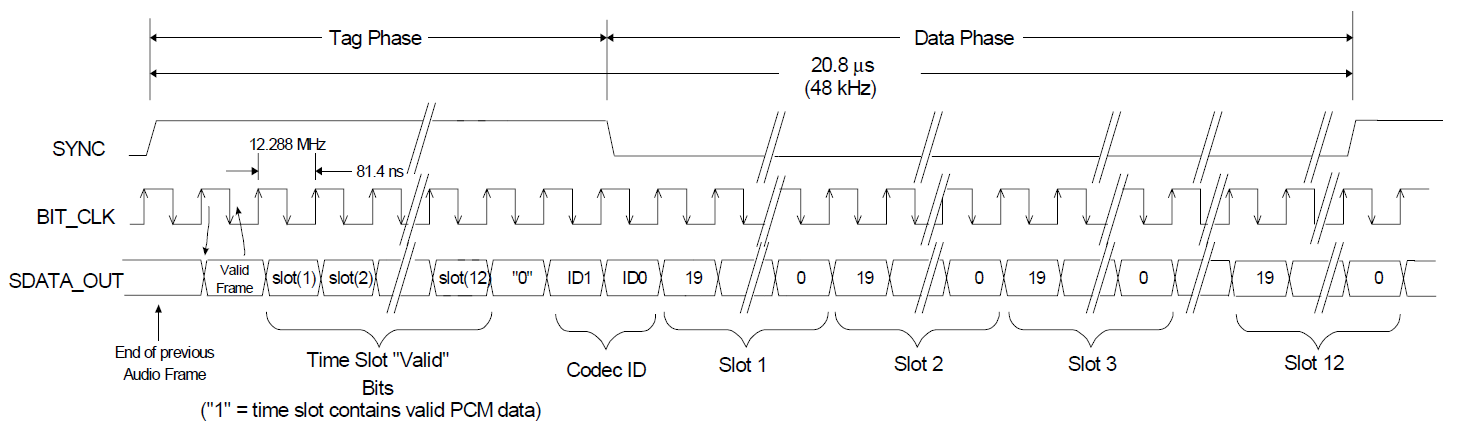
\includegraphics[width=6in]{ac97_framing_detail}
		\caption{Framing for AC97 with Timing Details}
	\end{center}
\end{figure}

\subsection{Sending the Frame Tag (Slot 0)}

The bits in the tag (slot 0) are indicate which, if any, of the other slots in the frame are valid. The tag bits are assigned as follows:

\renewcommand{\arraystretch}{1.1}
\begin{center}
	\begin{tabular}{ | l | l | p{8cm} |}
		\hline
		\textbf{Bit} & \textbf{Description} & \textbf{Value} \\ \hline
		15 & Frame Valid & Should be 1 always  \\ \hline
		14 & Slot 1: Valid Register Address & Should be 1 if we are writing or reading from a control register in the codec  \\ \hline
		13 & Slot 2: Valid Register Data & Should be 1 if we are writing to a control register in the codec \\ \hline
		12 & Slot 3: PCM Left Channel Valid Data & Should be 1 if we have a sample to send to the codec  \\ \hline
		11 & Slot 4: PCM Right Channel Valid Data & Should be 1 if we have a sample to send to the codec  \\ \hline
		10-0 & Etc. Valid Bits & Should be set to 0 \\ \hline		
	\end{tabular}
\end{center}

\subsection{Setting Control Registers With Slots 1 and 2}
After you send the correct tag through \verb|SDATA_OUT|, you will then need to fill slots 1 and 2. These slots contain an address and a value which refer to some control register on the codec IC. The codec contains a multitude of registers which control various features (volume/gain, mute, etc.). Our controller will need to manipulate some registers to unmute the codec and to set the volume appropriately.

\textbf{You should refer to the codec datasheet, specifically the table on page 12} to get the details of these control registers. We have specified below the registers that you will need to manipulate.

\begin{center}
	\begin{tabular}{ | l | l | p{10cm} |}
		\hline
		\textbf{Reg Address} & \textbf{Description} & \textbf{Value} \\ \hline
		0x02 & Master Volume & Should unset the mute bit and set right and left volume \\ \hline
		0x04 & Headphone Volume & Should unset the mute bit and set right and left volume \\ \hline
		0x18 & PCM-Out Volume & Should unset the mute bit and set right and left volume \\ \hline
	\end{tabular}
\end{center}

In \textbf{slot 1}, the command register address needs to be specified as follows in 20 bits.
\begin{enumerate}
	\item \verb|Bit[19]| - Read/Write Command (1 = read, 0 = write)
	\item \verb|Bit[18:12]| - Control Register Address (64 16-bit locations, addressed on even byte boundaries)
	\item \verb|Bit[11:0]| - Set to 0
\end{enumerate}

The first bit (MSB) sampled by AC97 indicates whether the current control transaction in this frame is a read or write operation. The following 7 bit positions communicate the targeted control register address. The trailing 12 bits should be 0.

In \textbf{slot 2}, the command register data needs to be specified as follows in 20 bits:

\begin{enumerate}
	\item \verb|Bit[19:4]| - Control Register Write Data (16 bits)
	\item \verb|Bit[3:0]| - Set to 0
\end{enumerate}

If we are writing data to a register, you must send the data with the MSB first in the first 16 bits of slot 2. If you are reading data, the entire slot 2 must be filled with 0s.

\subsection{Sending Linear PCM (pulse code modulation) Samples in Slots 3 and 4}
The next 2 slots \textbf{(slots 3 and 4)} are used for sending the actual audio samples you want the codec to push to the headphone output. Remember that the samples must be transmitted MSB first and each sample is 20 bits wide. Also note that each sample is a signed integer encoded with 2s complement, so the total range is roughly $\pm 2^{19}$. Each sample represents the amplitude of the audio wave to be played.

Fill the remaining slots \textbf{(slots 5-12)} with all 0s for each 20-bit slot.

\subsection{Codec Timing}
The datasheet is useful for figuring out how the timing works with the codec. Pay close attention to the timing parameters and diagrams on \textbf{pages 6-7 of the datasheet} as your controller needs to be coded with those in mind.

Your controller will need to send bits on the rising edges of \verb|BIT_CLK|, and the codec will sample them on the falling edge of the \verb|BIT_CLK|. Recall, that the \verb|BIT_CLK| is provided by the codec.

\subsubsection{Codec Reset}
Your controller will have to perform a cold reset of the codec when it receives a reset signal from the FPGA board (when you press the \verb|CPU_RESET| button). The cold reset timing is critical, since if your controller doesn't hold the reset properly, the codec may lose its clock.

This timing diagram below is critical to understanding how to reset the codec.

\begin{figure}[hbt]
	\begin{center}
		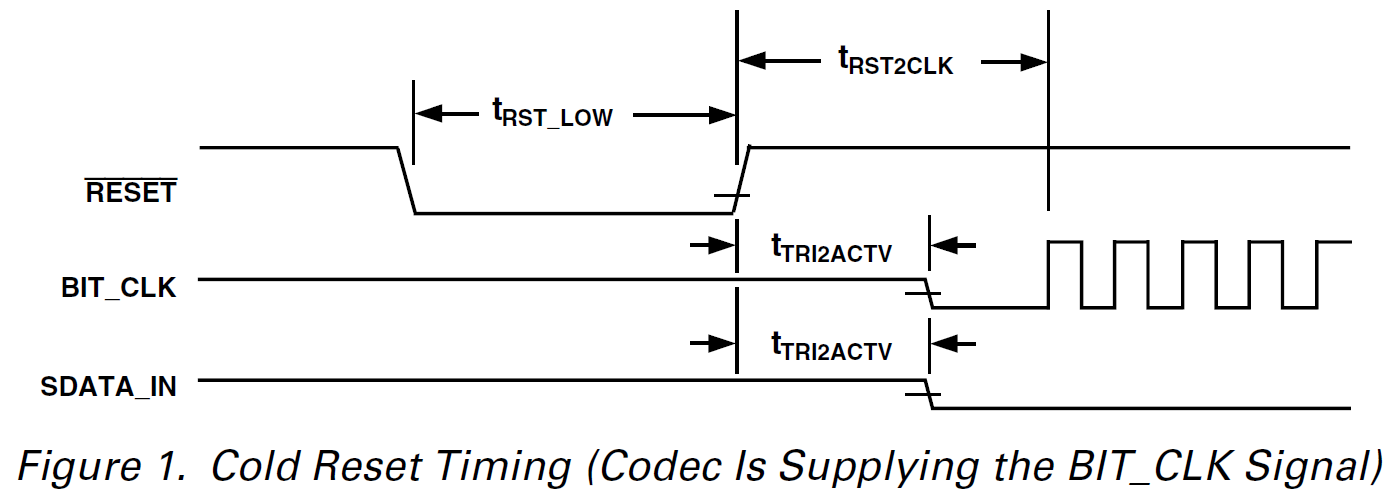
\includegraphics[width=6in]{ac97_codec_timing}
		\caption{Reset Timing Diagram from Datasheet}
	\end{center}
\end{figure}

You will notice from the diagram, that the reset signal that your controller will send to the codec is active low, which means that to assert the reset signal, you have to pull the line low. You will need to pull the reset signal low for at least $t_{RST\_LOW}$ which is defined in the datasheet. While the reset signal is being asserted, the codec will stop producing the \verb|BIT_CLK| and thus you cannot rely on it during reset; you must instead rely on a different clock to time the reset.

Once the reset signal has been asserted for the required time, after a delay of $t_{RST2CLK}$, the \verb|BIT_CLK| will begin to oscillate, after which the controller can begin transmitting frames to the codec. When the codec undergoes a cold reset, all its registers are set to their default values as specified in the datasheet.

\subsubsection{SYNC Signal for Frame Timing}
The codec needs a way to know when a frame is about to begin so that it can interpret its content appropriately. This is done using the \verb|SYNC| signal which is sent from your controller to the codec. You should assert \verb|SYNC| for a total duration of 16 \verb|BIT_CLK|s at the beginning of each audio frame. Refer back to Figure 3 in Section 3.2 to understand how the \verb|SYNC| signal should be asserted with each frame.

\section{Building the AC97 Controller}

Begin by copying files from previous labs.

WARNING: Specifically for this lab, DO NOT use the rst signal inside the synchronizer, debouncer, and edge detector modules. Since the rst signal is generated by these modules detecting a reset button press and is then fed back to these modules, it can cause an undesirable feedback loop especially for the ac97 controller.

WARNING: for simulation to work properly, you may have to forcefully reset the debouncer's 2D saturating counter reg. If you get Xs in your simulation for the entire time for the saturating counter, add this code to the debouncer Verilog file.

    initial begin:INITIALIZE\_SAT\_COUNTER
    integer k;
    for (k = 0; k < width; k = k + 1) begin
    saturating\_counter[k] <= 0;
    end
    end

WARNING: Do not assert your ac97 controller's codec reset signal (reset\_b) longer than tRSTLOW. If you assert cold resets to the codec IC too often it will lose its clock and refuse to operate correctly. If this happens to you, just run make impact again to restore the ac97 codec.

WARNING: If you make sync, reset, and sdata\_out registers in the controller, they must ALL be registers and they should march in line.

WARNING: Attenuate the audio using the control registers otherwise you may destroy your headphones by blowing the drivers with too much power!!! Check with the TA if you are unsure if you have attenuated your volume levels appropriately.

\subsection{Testing}

\section{Connect the music\_streamer and tone\_generator}

\subsection{Testing}

\section{Try it on the FPGA!}

\section{Conclusion + Checkoff}
You are done with lab 6! Please write down any and all feedback and criticism of this lab and share it with the TA. This is a brand new lab and we welcome everyone's input so that it can be improved.

\subsection{Checkoff Tasks}

\begin{enumerate}
	\item Show the TA your working AC97 controller by demonstrating the state machine in the \verb|music_streamer| working and sending audio to the AC97 codec.
\end{enumerate}

\end{document}